\documentclass[11pt, oneside]{article}   	% use "amsart" instead of "article" for AMSLaTeX format
\usepackage{geometry}                		% See geometry.pdf to learn the layout options. There are lots.
\geometry{letterpaper}                   		% ... or a4paper or a5paper or ... 
%\geometry{landscape}                		% Activate for for rotated page geometry
%\usepackage[parfill]{parskip}    		% Activate to begin paragraphs with an empty line rather than an indent
\usepackage{graphicx}				% Use pdf, png, jpg, or eps� with pdflatex; use eps in DVI mode
								% TeX will automatically convert eps --> pdf in pdflatex		
\usepackage{amssymb}
\usepackage{amsmath}
\usepackage{parskip}
\usepackage{color}
\usepackage{hyperref}

\title{Calculus of variations}
%\author{The Author}
%\section{}
%\subsection*{}
\date{}							% Activate to display a given date or no date

\graphicspath{{/Users/telliott_admin/Dropbox/Tex/png/}}
% \begin{center} 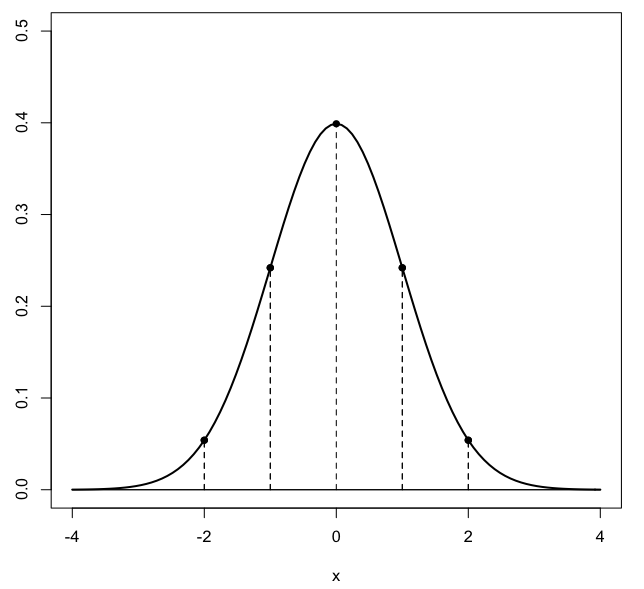
\includegraphics [scale=0.4] {gauss3.png} \end{center}
\begin{document}
\maketitle
\Large
Consider two points in the $xy$-plane $(x_1,y_1)$ and $(x_2,y_2)$, and the paths that connect them.  One path is the shortest path, namely a straight line.  Our goal is to prove that.

There are many possible paths, any one of which we could try to write as $y=f(x)$ or to use fewer symbols we write $y = y(x)$.

As you know, any small element of the path $ds$ is (by Pythagoras)
\[ ds = \sqrt{dx^2 + dy^2} \]
Factoring out $dx$ we get
\[ ds = \sqrt{1 + (\frac{dy}{dx})^2} \ dx =  \sqrt{1 + y'(x)^2} \ dx \]
The total path length is
\[ L = \int_{x_1}^{x_2} \sqrt{1 + y'(x)^2} \ dx \]
The unknown is the function $y = y(x)$.  The principle is that we will find $y(x)$ such that any infinitesimal change in $y(x)$ makes no difference in the length, to first order.  We say that such a path makes the integral \textbf{stationary}.

\subsection*{Fermat's principle}
The problem can be made slightly harder by including some function $f(x,y)$ under the integral.  For example, consider the path taken by a light beam between two points.  If the refractive index varies with position, then the path will not be a straight line.  Instead, light takes the path that takes the \emph{least time}.
\[ \text{time} \ = \int_1^2 dt = \int_1^2 \frac{ds}{v} \]
where $v \ dt = ds$ and the velocity $v=c/n$ so
\[ \text{time} \ = \int_1^2 dt = \int_1^2 \frac{ds}{v} = \frac{1}{c}  \int_1^2 n \ ds  \]
$n$ is a function $n(x,y)$, and we substitute for $ds$:
\[ \text{time} \ = \frac{1}{c}  \int_{x_1}^{x_2} n(x,y) \ \sqrt{1 + y'(x)^2} \ dx \]
Since for any parametrized curve (which is all we can really deal with), $y = y(x)$, the function $n(x,y)$ is really only dependent on $x$ and this is a single integral over $x$.

\subsection*{generally}
We will have some integral over $x$ where the integrand is a function that depends on $x$, on $y(x)$ and on $y'(x)$ so we write
\[ S = \int_{x_1}^{x_2} f\ [ \ y(x), y'(x), x \ ] \ dx \]
where $y(x)$ is an unknown curve and we seek the $y(x)$ which makes the integral stationary.

Let us denote the correct solution to the problem as $y(x)$ and all the other "wrong" curves as $Y(x)$ and then
\[ Y(x) = y(x) + \eta(x) \]
$\eta$ is a term that contains all the extra length of a wrong path $Y$ compared to the shortest path $y$.  We are only interested in paths $Y(x)$ that pass through the endpoints $(x_1,y_1)$ and $(x_2,y_2)$.  At those points $\eta$ must be zero because $Y = y$ there.
\[ \eta(x_1) = \eta(x_2) = 0 \]
As Taylor says, "there are infinitely many choices for the difference $\eta(x)$, for example we could choose $\eta = (x - x_1)(x - x_2)$ or $\sin \ [ \pi (x - x_1)/(x_2 - x_1) \ ]$."

The function $\eta$ will have something that makes the difference in $Y(x) - y(x)$.  Let us parametrize those things that make the difference and factor them out into a parameter $\alpha$ so that
\[ Y(x) = y(x) + \alpha \eta(x) \]
The integral $S$ now depends on $\alpha$.  The curve $y(x)$ is obtained by setting $\alpha = 0$.  Our problem is now to make sure that $S(\alpha)$ is a minimum when $\alpha = 0$.  We write
\[ S(\alpha) =  \int_{x_1}^{x_2} f\ [ \ Y(x), Y'(x), x \ ] \ dx \]
\[ =  \int_{x_1}^{x_2} f\ [ \ y + \alpha \eta(x), y' + \alpha \eta'(x), x \ ] \ dx \]
Notice that although $\eta$ depends on $x$, $\alpha$ does not.

Next, we want to differentiate $S$ with respect to $\alpha$ and set that derivative equal to zero.  Differentiating the integrand:
\[ \frac{\partial}{\partial \alpha}  f\ [ \ y + \alpha \eta(x), y' + \alpha \eta'(x), x \ ] \ = \eta \ \frac{\partial f}{\partial y}  + \eta' \ \frac{\partial f}{\partial y'} \]
I don't understand the previous step.

But given this
\[ \frac{dS}{d \alpha} = \int_{x_1}^{x_2} \frac{\partial f}{\partial \alpha} \ dx \]
\[ = \int_{x_1}^{x_2} (  \eta \ \frac{\partial f}{\partial y}  + \eta' \ \frac{\partial f}{\partial y'} ) \ dx \]

This condition must be true for any choice of the path.

Now he says, we will rewrite the second term on the right using integration by parts.
\[ \int_{x_1}^{x_2}  \eta' \ \frac{\partial f}{\partial y'} \ dx = \eta(x) \frac{\partial f}{\partial y'} \ \bigg |_{x_1}^{x_2} - \int_{x_1}^{x_2} \eta(x) \frac{d}{dx} \ \frac{\partial f}{\partial y'}  \ dx \]
Because $\eta(x_1) = \eta(x_2) = 0$, the first term is zero and we have then:
\[ \int_{x_1}^{x_2}  \eta' \ \frac{\partial f}{\partial y'} \ dx = - \int_{x_1}^{x_2} \eta(x) \frac{d}{dx} \ \frac{\partial f}{\partial y'}  \ dx \]

Substitute back into the derivative and set it equal to zero:
\[  \int_{x_1}^{x_2} \eta(x) ( \frac{\partial f}{\partial y}  -  \frac{d}{dx} \ \frac{\partial f}{\partial y'} )  \ dx = 0 \]
Since this must be true for any choice of $\eta(x)$, the term in parentheses must be zero (at least if the functions involved are continuous functions, and our examples will be).  So we have finally
\[  \frac{\partial f}{\partial y}  =  \frac{d}{dx} \ \frac{\partial f}{\partial y'} \]
which is the Euler-Lagrange equation.

\subsection*{examples}
In the shortest path between two points we had
\[ y'(x) = \sqrt{1 + y'(x)^2} \]

\end{document}  